
\documentclass[11pt]{article}

\usepackage{alltt}
\usepackage{graphicx}
\usepackage{subfigure}
\usepackage[dvips]{epsfig}
% New mathematical facilities like \mathbb, \big, and \mapsto
\usepackage{amssymb}
% Defines page size and margins.
%
%   Preamble
%
%
%   The parameter oddsidemargin (evensidemargin) is one inch 
%   less than the distance from the edge of the paper to the 
%   left margin of the text on right-hand (left-hand) pages. 
%
\setlength{\textwidth}{6.0in}
\setlength{\oddsidemargin}{23pt}
\setlength{\evensidemargin}{23pt}
\setlength{\topmargin}{-0.5in}
\setlength{\textheight}{8.5in}

%   Some abbreviations

\newcommand{\grad}{\nabla}
\newcommand{\bull}{\vrule height 1.8ex width 1.0ex depth 0ex}
\newcommand{\half}{{\textstyle{\frac{1}{2}}}}
\newcommand{\Ref}[1]{\mbox{\rm{(\ref{#1})}}}
\newcommand{\qed}{$ \blacksquare $ \medskip}
\newcommand{\lt}{<}
\newcommand{\gt}{>}
%
%   Enviroments theorem lemma and algorithm are created, and all
%   three are numbered as in theorem.
%
\newtheorem{theorem}{Theorem}
\newtheorem{lemma}[theorem]{Lemma}
\newtheorem{corollary}[theorem]{Corollary}
\newtheorem{algorithm}[theorem]{Algorithm}
\newtheorem{definition}[theorem]{Definition}
\newtheorem{assumption}[theorem]{Assumption}
%
%   The numbering below can be done with the numinsec style
%   provided by SIAM.
%
%   The theorem numbers are defined to be of the form section#.theorem#
%
\renewcommand{\thetheorem}{\thesection.\arabic{theorem}}
%
%   Defines the equation number to be of the form section#.equation#
%
%   \renewcommand{\theequation}{\thesection.\arabic{equation}}
%
%   Defines the figure and table numbers to be of the form 
%   section#.figure# and section#.table#
%
\renewcommand{\thefigure}{\thesection.\arabic{figure}}
\renewcommand{\thetable}{\thesection.\arabic{table}}


% Redefines the size of the section headings.
\usepackage{../sty/art11mod}
% The float package is described in page 146 of the LaTeX companion.
\usepackage{../sty/float}
% Numbers equations,... consecutively within sections.
\usepackage{../sty/numinsec}
% The bar package is described in page 283 of the LaTeX companion.
\usepackage{../sty/bar}
% The url package is intended for email addresses, hypertext links, ...
\usepackage{../sty/url}

%\usepackage[first]{draftcopy}
%\usepackage{subfigure}

% New commands
\newcommand{\QED}{~\rule[-1pt] {8pt}{8pt}\par\medskip}
\newcommand{\R}{\mbox{${\mathbb R}$}}
\newcommand{\Note}{\marginpar[$\Rightarrow$]{$\Leftarrow$}}
% Renewing commands
\renewcommand{\thefootnote}{\fnsymbol{footnote}}
% Algorithm floating environment.
\newfloat{Algorithm}{thp}{loa}[section]

% Calligraphic letter abbreviations.

\newcommand{\cA} {\mbox{$\cal A$}}
\newcommand{\cB} {\mbox{$\cal B$}}
\newcommand{\cD} {\mbox{$\cal D$}}
\newcommand{\cF} {\mbox{$\cal F$}}
\newcommand{\cI} {\mbox{$\cal I$}}
\newcommand{\pg}  {\overline{g}}
\newcommand{\tc}  {T_{\Omega}}
\newcommand{\tck} {T_{\Omega}}
\newcommand{\tcc} {T_{\Omega}}
\newcommand{\comment}[1]{{}}
\newcommand{\proof}[1]{{\it Proof.} #1 \QED}

%\newcommand{\example}[2]{{\it Example #1.}  #2 \QED}

\newtheorem{example}{Example}

\begin{document}
\setlength{\baselineskip}{15pt}

%  \pagestyle {empty}
%  
\vspace{1.75in}

\begin{center}

ARGONNE NATIONAL LABORATORY

9700 South Cass Avenue

Argonne, Illinois  60439

\vspace{1.5in}

{\Large
{\bf 
TAO 3.9 Users Manual
}
}

\vspace{.5in}

{\bf Alp Dener \\ Todd Munson \\ Jason Sarich \\ Stefan Wild \\ Steven Benson \\ Lois Curfman McInnes}

\vspace{.5in}

Mathematics and Computer Science Division

\vspace{.25in}

Technical Memorandum ANL/MCS-TM-322

\vspace{.25in}

This manual is intended for use with TAO version 3.9

\vspace{1.0in}

\today
\end{center}

\vspace{0.75in}

\par\noindent
This product includes software produced by UChicago Argonne, LLC under 
Contract No. DE-AC02-06CH11357 with the Department of Energy.

%  \newpage
%  \mbox{}
%  \newpage

\begin{center}

{\large \bf A Limited Memory Variable Metric Method in Subspaces and 
Bound Constrained Optimization Problems\footnotemark}

%{\large \bf A Limited Memory Variable Metric Method for Bound Constrained
% Optimization Problems\footnotemark}

{\bf Steven J. Benson  and
Jorge J. Mor\'e}

\end{center}

% I THINK WE NEED TO EXPAND THE ABSTRACT AND FIRST PARAGRAPH TO
% STATE THAT WE HAVE RESULTS PERTAINING TO REDUCED SPACE BFGS METHODS
% IN GENERAL.  THEN WE USE THIS THEORY TO PROVIDE INSIGHT INTO OUR METHOD

% ALSO THE TITLE IS VAGUE.  IT IS ALMOST THE SAME TITLE USED BY
% BYRD, NOCEDAL, ET AL FOR THEIR TECHNICAL REPORT


\footnotetext
{ This work was supported by the Mathematical, Information, and
Computational Sciences Division subprogram of the Office of Advanced
Scientific Computing, U.S. Department of Energy, under Contract
W-31-109-Eng-38.}

\begin{abstract}

We describe an algorithm for solving nonlinear optimization problems
with lower and upper bounds that constrain the variables.  The algorithm
uses projected gradients to construct a limited memory BFGS matrix
and determine a step direction.  The algorithm has been implemented
and distributed as part of the Toolkit for Advanced Optimization (TAO).
We include numerical results demonstrate is effectiveness 
on a set of large test problems and
its scalability to multiple processors.

\end{abstract}

%  \noindent
%  {\bf Key words. } 
%  large-scale optimization,
%  gradient projection,
% limited memory method
% bound constrained optimization
% nonlinear optimization
% quasi Newton methods,
% BFGS methods,
% reduced space methods

%
%  Introduction to PETSc
%
%
% Note that we use a modified version of report.sty, so that tables and
% figures are numbered consecutively throughout the document (not by
% chapters).  
%
\documentclass[twoside,12pt]{../sty/report_petsc}

\usepackage{makeidx,xspace}
\usepackage[bookmarksopen,colorlinks]{hyperref}
\usepackage{color}
\input pdfcolor.tex     

\usepackage[pdftex]{graphicx}

%\usepackage{psfig}
\usepackage{../sty/verbatim}
\usepackage{../sty/tpage}
\usepackage{../sty/here}
\usepackage{../sty/anlhelper}
\usepackage{../sty/trl}

\setlength{\textwidth}{6.5in}
\setlength{\oddsidemargin}{0.0in}
\setlength{\evensidemargin}{0.0in}
\setlength{\textheight}{9.2in}
\setlength{\topmargin}{-.8in}

\newcommand{\findex}[1]{\index{FUNCTION #1}}
\newcommand{\sindex}[1]{\index{#1}}
 
% Defines the environment where design issues are discussed. In the manual
% version of this report, these regions are ignored.
\def\design{\medskip \noindent Design Issue:\begin{em}}
\def\enddesign{\end{em} \medskip}
% Manual version:
% \def\design{\comment}
% \def\enddesign{\endcomment}

% Print DRAFT in large letters across every page
% \special{!userdict begin /bop-hook{gsave 200 70 translate
% 65 rotate /Times-Roman findfont 216 scalefont setfont
% 0 0 moveto 0.95 setgray (DRAFT) show grestore}def end}

% Defines that we're doing the short intro part, not the whole manual,
% used in part1.tex.
\def\shortintro{*}
\renewcommand{\cite}[1]{}
\def\thesection {$\!\!\!\!$}

\begin{document}

\begin{center}
$\!$
\vspace{1.0cm}
\thispagestyle{empty}

{\huge \bf Introduction to PETSc}\\ 
\vspace{0.5cm}
{\LARGE (Part I of the PETSc Users Manual)} \\
\vspace{1.5cm}
{\large \em Satish Balay\\Kris Buschelman\\Victor Eijkhout\\William Gropp\\Dinesh Kaushik\\Matt Knepley\\Lois Curfman McInnes\\Barry Smith\\Hong Zhang\\
\medskip \medskip
Mathematics and Computer Science Division\\
Argonne National Laboratory\\
9700 South Cass Avenue\\
Argonne, IL 60439-4844\\
\medskip
 2008}
\end{center}

\vspace{1.0cm}

% Abstract for TAO Users Manual

\addcontentsline{toc}{chapter}{Preface}
\section*{Preface}

The Toolkit for Advanced Optimization (TAO) focuses on the development
of algorithms and software for the solution of large-scale optimization 
problems on high-performance architectures.  Areas of interest include 
unconstrained and bound-constrained optimization, nonlinear least squares 
problems, optimization problems with partial differential equation 
constraints, and variational inequalities and complementarity 
constraints.

The development of TAO was motivated by the scattered support for
parallel computations and the lack of reuse of external toolkits in
current optimization software.  Our aim is to produce high-quality 
optimization software for computing environments ranging from 
workstations and laptops to massively parallel high-performance 
architectures.  Our design decisions are strongly motivated by 
the challenges inherent in the use of large-scale distributed 
memory architectures and the reality of working with large, 
often poorly structured legacy codes for specific 
applications.

This manual describes the use of TAO 2.2.0.  Since TAO is still under 
development, changes in usage and calling sequences may occur.  TAO 
is fully supported; see the the web site \url{http://www.mcs.anl.gov/tao} 
for information on contacting the developers.

%%% Local Variables: 
%%% mode: latex
%%% TeX-master: "manual_tex"
%%% End: 



\noindent {\bf Note:} This document serves as the first section of the {\em PETSc Users
Manual}, which elaborates on the use and design of PETSc. The
manual and is available in its entirety via the World Wide Web at
the PETSc home page, {\tt http://www.mcs.anl.gov/petsc}.
When referencing PETSc, please do 
not refer to this document. Instead reference the following: Satish
Balay, Kris Buschelman, Victor Eijhout, William Gropp, Dinesh Kaushik, 
Lois Curfman McInnes, Barry Smith and Hong Zhang.  {\em
PETSc Users Manual}, Technical Report ANL-95/11 - Revision 3.0.0,
Argonne National Laboratory, 2008.

%
% Acknowledgements for users manual
\newpage
% Acknowledgements for PETSc Users Manual
%
% These are also listed on the PETSc homepage, so if you add something here
% add it to the home page also
%
\noindent {\bf Acknowledgments:}

\medskip \medskip \noindent
We thank all PETSc users for their many suggestions, bug reports, and
encouragement.  We especially thank Victor Eijkhout, David Keyes, and
Matthew Knepley for their valuable comments on the source code,
functionality, and documentation for PETSc.


\vspace{.3in}
\noindent
Some of the source code and utilities in PETSc (or software used by PETSc)
have been written by 
\begin{itemize}
  \item Mark Adams, scalability features of MPIBAIJ matrices,
  \item Allison Baker, the flexible GMRES code,
  \item Tony Caola, the SPARSEKIT2 ilutp() interface,
  \item Chad Carroll, Win32 graphics,
  \item Cameron Cooper, portions of the VecScatter routines, 
  \item Victor Eijkhout, KSP type BICG, VecPipeline() and VecXXXBegin()/End() routines, 
  \item Paulo Goldfeld, balancing Neumann-Neumann preconditioner,
  \item Matt Hille, 
  \item Matthew Knepley,
  \item Domenico Lahaye, the interface to John Ruge and Klaus Stueben's AMG,
  \item Peter Mell, portions of the DA routines,
  \item Todd Munson, the LUSOL (sparse solver in MINOS) interface,
  \item Wing-Lok Wan, the ILU portion of BlockSolve95,
  \item Liyang Xu, the interface to PVODE.
\end{itemize}

\vspace{.3in}
\noindent
PETSc uses routines from 
\begin{itemize}
  \item BLAS
  \item LAPACK
  \item LINPACK      matrix factorization and solve; converted to C using {\tt f2c} and then 
                      hand-optimized for small matrix sizes, for block matrix data structures,
  \item MINPACK      sequential matrix coloring routines for finite difference Jacobian
                       evaluations; converted to C using {\tt f2c},
  \item SPARSPAK     matrix reordering routines, converted to C using {\tt f2c},
  \item SPARSEKIT2   written by Yousef Saad, iludtp(), converted to C using {\tt f2c}. These routines 
                     are copyrighted by Saad under the GNU copyright, see \trl{${PETSC_DIR}/src/mat/impls/aij/seq/ilut.c}.
  \item libtfs the efficient, parallel direct solver developed by Henry Tufo and Paul Fischer.
\end{itemize}


\vspace{.3in}
\noindent
PETSc interfaces to the following external software:
\begin{itemize}
  \item AMG          the algebraic multigrid code of John Ruge and Klaus Stueben,
                     \trllink{http://www.mgnet.org/mgnet-codes-gmd.html}{http://www.mgnet.org/mgnet-codes-gmd.html}
  \item BlockSolve95 for parallel ICC(0) and ILU(0) preconditioning,
                     \trllink{http://www.mcs.anl.gov/blocksolve}{http://www.mcs.anl.gov/blocksolve},
  \item ESSL         IBM's math library for fast sparse direct LU factorization,
  \item LUSOL        sparse LU factorization code (part of MINOS) developed by Michael Saunders,
                      Systems Optimization Laboratory, Stanford University,
                     \trllink{http://www.sbsi-sol-optimize.com/}{http://www.sbsi-sol-optimize.com/},
  \item Matlab       
  \item ParMeTiS      parallel graph partitioner, \trllink{http://www-users.cs.umn.edu/~karypis/metis/}{http://www-users.cs.umn.edu/~karypis/metis/},
  \item PVODE        parallel ODE integrator, \trllink{http://www.llnl.gov/CASC/PVODE}{http://www.llnl.gov/CASC/PVODE},
  \item SPAI         for parallel sparse approximate inverse preconditiong, 
                     \trllink{http://www.sam.math.ethz.ch/~grote/spai/}{http://www.sam.math.ethz.ch/~grote/spai/}.
\end{itemize}
These are all optional packages and do not need to be installed to use PETSc.




\newpage
% Include only Part 1 of users manual 
\section{Introduction}
% $Id: part1.tex,v 1.146 2001/08/22 18:03:15 balay Exp $ 

% --------------------------------------------------------------------
%
%                            PART 1
%
%   This introductory PETSc information is included in 
%   both manual.tex and intro.tex.
%
% --------------------------------------------------------------------

\label{sec_gettingstarted}

The Portable, Extensible Toolkit for Scientific Computation (PETSc)
has successfully demonstrated that the use of modern programming
paradigms can ease the development of large-scale scientific
application codes in Fortran, C, and C++.  Begun several years ago,
the software has evolved into a powerful set of tools for the
numerical solution of partial differential equations and related problems 
on high-performance computers.

PETSc consists of a variety of libraries (similar to classes in C++),
which are discussed in detail in Parts II and III of the users manual.
Each library manipulates a particular family of objects (for instance,
vectors) and the operations one would like to perform on the objects.
The objects and operations in PETSc are derived from our long 
experiences with scientific computation. Some of the PETSc modules deal with 
\begin{itemize} 
\item index sets, including permutations, for indexing into vectors, renumbering, etc;
\item vectors;
\item matrices (generally sparse);
\item distributed arrays (useful for parallelizing regular grid-based 
      problems);
\item Krylov subspace methods;
\item preconditioners, including multigrid and sparse direct solvers;
\item nonlinear solvers; and
\item timesteppers for solving time-dependent (nonlinear) PDEs.
\end{itemize}
Each consists of an abstract interface 
(simply a set of calling sequences) and one or more implementations 
using particular data structures. Thus, PETSc provides clean and 
effective codes for the various phases of solving PDEs, with a uniform 
approach for each class of problems.  This design
enables easy comparison and use of different algorithms (for example,
to experiment with different Krylov subspace methods, preconditioners,
or truncated Newton methods).
Hence, PETSc provides a rich environment for modeling scientific
applications as well as for rapid algorithm design and prototyping.

The libraries enable easy customization and extension of both algorithms
and implementations.  This approach promotes code reuse and
flexibility, and separates the issues of parallelism from the choice
of algorithms.  The PETSc infrastructure creates a
foundation for building large-scale applications.

It is useful to consider the interrelationships among different
pieces of PETSc.  Figure \ref{fig_1} is a diagram of some 
of these pieces; Figure \ref{fig_2} presents
several of the individual parts in more detail.
These figures illustrate the library's hierarchical organization,
which enables users to employ the level of abstraction that is most 
appropriate for a particular problem.  
\begin{figure}[hbt]
%\centerline{ \pdfximage height 3.4in {petscwww.pdf} \pdfrefximage \pdflastximage}
\centerline{ 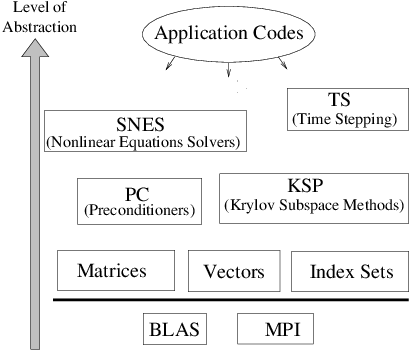
\includegraphics{petscwww}}
%\centerline{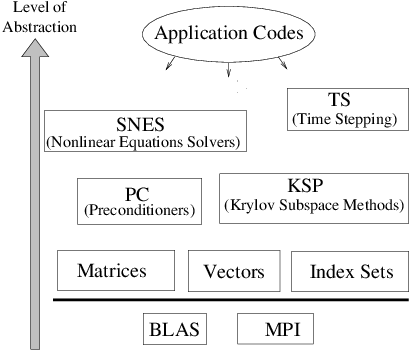
\psfig{file=petscwww.ps,angle=270,height=3.4in}}
% \centerline{\psfig{file=petsc_pt.eps,angle=0,height=4in,width=5in}}
\caption{Organization of the PETSc Libraries}
\label{fig_1}
\end{figure}

\begin{figure}[hbt]
\centerline{ 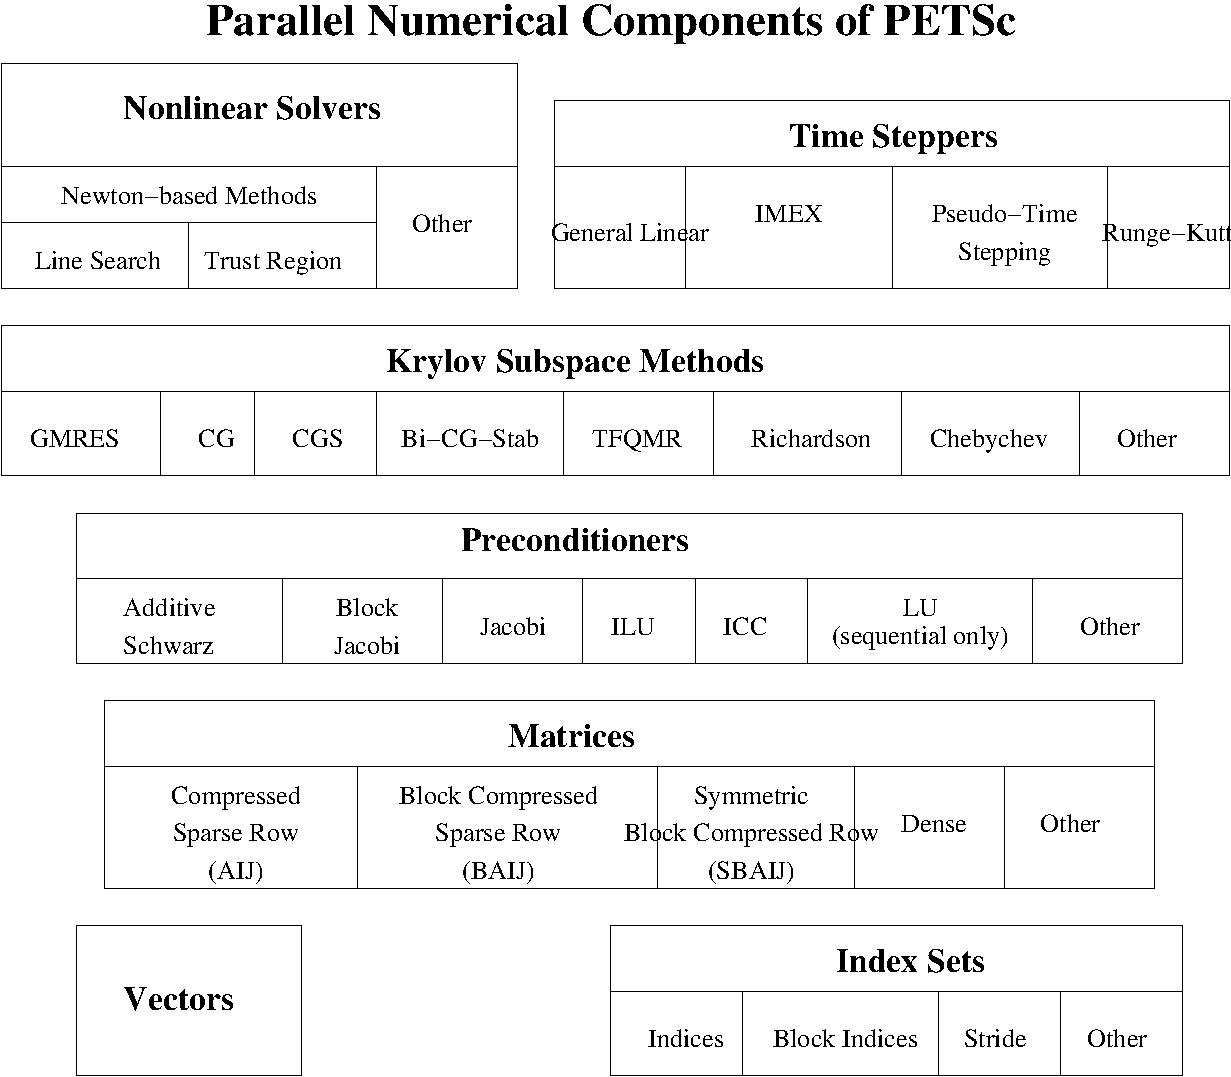
\includegraphics{zoom}}
%\centerline{\psfig{file=zoom_ls.ps,angle=270,height=3.4in}}
\caption{Numerical Libraries of PETSc}
\label{fig_2}
\end{figure}

\section{Suggested Reading}

The manual is
divided into three parts:
\begin{itemize}
\item Part I - Introduction to PETSc
\item Part II - Programming with PETSc
\item Part III - Additional Information
\end{itemize}

Part I describes
the basic procedure for using the PETSc library and presents two
simple examples of solving linear systems with PETSc.  This section
conveys the typical style used throughout the library and enables the
application programmer to begin using the software immediately.
Part I is also distributed separately for individuals interested in an 
overview of the PETSc software, excluding the details of library usage.
Readers of this separate distribution of Part I should note that all
references within the text to particular chapters and sections 
indicate locations in the complete users manual.

Part II explains in detail the use of the various PETSc libraries,
such as vectors, matrices, index sets, linear and nonlinear
solvers, and graphics.  Part III describes a variety of useful
information, including profiling, the options database, viewers, error
handling, makefiles, and some details of
PETSc design.

\nocite{efficient}

PETSc has evolved to become quite a comprehensive package, and therefore the
{\em PETSc Users Manual} can be rather intimidating for new users. We
recommend that one initially read the entire document before proceeding with
serious use of PETSc, but bear in mind that PETSc can be used efficiently
before one understands all of the material presented here. Furthermore, the
definitive reference for any PETSc function is always the online manualpage.

\medskip \medskip

Within the PETSc distribution, the directory \trl{${PETSC_DIR}/docs}
contains all documentation.
Manual pages for all PETSc functions can be
accessed on line at
\begin{tabbing}
  http://www.mcs.anl.gov/petsc/docs/
\end{tabbing}
The manual pages
provide hyperlinked indices (organized by
both concepts and routine names) to the tutorial examples and enable
easy movement among related topics.  

Emacs users may find the
{\em etags} option to be extremely useful for exploring the PETSc
source code.  Details of this feature are provided in
Section~\ref{sec_emacs}. 

The file \trl{manual.pdf} contains
the complete {\em PETSc Users Manual} in the portable document format (PDF), 
while \trl{intro.pdf} 
includes only the introductory segment, Part I.  \sindex{installing PETSc} 
The complete PETSc distribution, users
manual, manual pages, and additional information are also available via
the PETSc home page at
\trllink{http://www.mcs.anl.gov/petsc}{http://www.mcs.anl.gov/petsc}.  
The PETSc home page also
contains details regarding installation, new features and changes in recent
versions of PETSc, machines that we currently support, a
troubleshooting guide, and a FAQ list for frequently asked questions.

\medskip\medskip

\noindent{\bf Note to Fortran Programmers}: In most of the  
manual, the examples and calling sequences are given for the C/C++
family of programming languages.  We follow this convention because we
recommend that PETSc applications be coded in C or C++.
However, pure Fortran programmers can use most of the
functionality of PETSc from Fortran, with only minor differences in
the user interface.  Chapter \ref{ch_fortran} provides a discussion of the
differences between using PETSc from Fortran and C, as well as several
complete Fortran examples.  This chapter also introduces some
routines that support direct use of Fortran90 pointers.

%-----------------------------------------------------------------------------
\section{Running PETSc Programs}
\label{sec_running}

Before using PETSc, the user must first set the environmental variable
\trl{PETSC_DIR}, \findex{PETSC_DIR} indicating the full path of the PETSc home
directory.  For example, under the UNIX C shell a command of the form
\begin{tabbing}
   setenv PETSC\_DIR \$HOME/petsc
\end{tabbing}
 can be placed in the user's \trl{
.cshrc} file.  In addition, the user must set the environmental
variable {\trl{PETSC_ARCH}} to specify the architecture (e.g., rs6000,
solaris, IRIX, etc.)  on which PETSc is being used.  The utility
 \trl{${PETSC_DIR}/bin/petscarch} can be used for this purpose.  For example,
\begin{tabbing}
   setenv PETSC\_ARCH `\$PETSC\_DIR/bin/petscarch`
\end{tabbing}
can be placed in a \trl{.cshrc} file.  Thus, even if several machines of different
types share the same filesystem, \trl{PETSC_ARCH} will be set correctly
when logging into any of them. 

All PETSc programs use the MPI (Message Passing Interface) standard
for message-passing communication \cite{MPI-final}.  Thus, to execute
PETSc programs, users must know the procedure for beginning MPI jobs
on their selected computer system(s).  For instance, when using the
MPICH implementation of MPI \cite{mpich-web-page} and many others, the following
command initiates a program that uses eight processors:
\findex{mpirun} \sindex{running PETSc programs} 
\begin{tabbing}
   mpirun -np 8 petsc\_program\_name petsc\_options
\end{tabbing}

PETSc also comes with a script 
\begin{tabbing}
   \${PETSC\_DIR}/bin/petscmpirun -np 8 petsc\_program\_name petsc\_options
\end{tabbing}
that uses the information set in \trl{${PETSC_DIR}/bmake/${PETSC_ARCH}/packages} to 
automatically use the correct \trl{mpirun} for your configuration.

All PETSc-compliant programs support the use of the \trl{-h}
\findex{-h} or \trl{-help} option as well as the \trl{-v} \findex{-v}
or \trl{-version} option. 


Certain options are supported by all PETSc programs.  We list a few 
particularly useful ones below; a complete list can be obtained by 
running any PETSc program with the option \trl{-help}.
\begin{itemize}
\item \trl{-log_summary} - summarize the program's performance
\item \trl{-fp_trap} - stop on floating-point exceptions; \findex{-fp_trap}
      for example divide by zero
\item \trl{-trdump} - enable memory tracing; dump list of unfreed memory 
      at conclusion \findex{-trdump} of the run
\item \trl{-trmalloc} - enable memory tracing (by default this is 
      activated for versions of PETSc using BOPT=g*)
\item \trl{-start_in_debugger} \trl{[noxterm,gdb,dbx,xxgdb]} \trl{[-display name]} 
     - start all processes in debugger \findex{-start_in_debugger} \sindex{debugger}
\item \trl{-on_error_attach_debugger}  \trl{[noxterm,gdb,dbx,xxgdb]}
      \trl{[-display name]} - \findex{-on_error_attach_debugger}start debugger only on encountering an error
\end{itemize}
See Section \ref{sec_debugging} for more information on debugging PETSc programs.

%-----------------------------------------------------------------------------
\section{Writing PETSc Programs}
\label{sec_writing}

Most PETSc programs begin with a call to \findex{PetscInitialize()}
\begin{tabbing}
  PetscInitialize(int *argc,char ***argv,char *file,char *help);
\end{tabbing} 
which initializes PETSc and MPI.  The arguments \trl{argc} and 
\trl{argv} are the command line arguments delivered in all C and C++
programs. \sindex{command line arguments} The argument \trl{file}
optionally indicates an alternative name for the PETSc options file,
\trl{.petscrc}, which resides by default in the user's home directory.
Section \ref{sec_options} provides details regarding
this file and the PETSc options database, which can be used for runtime
customization. The final argument, \trl{help}, is an optional
character string that will be printed if the program is run with the
\trl{-help} option.  In Fortran the initialization command has the form
\begin{tabbing}
   call PetscInitialize(character(*) file,integer ierr)
\end{tabbing} 
\trl{PetscInitialize()} automatically calls \trl{MPI_Init()} if MPI
has not been not previously initialized. In certain \findex{MPI_Init()}
circumstances in which MPI needs to be initialized directly (or is
initialized by some other library), the user can first call 
\trl{MPI_Init()} (or have the other library do it), and then call
\trl{PetscInitialize()}.
By default, \trl{PetscInitialize()} sets the PETSc ``world''
communicator, given by \trl{PETSC_COMM_WORLD}, to \trl{MPI_COMM_WORLD}.
\findex{PETSC_COMM_WORLD}

For those not familar with MPI, a {\em communicator} is a way of
indicating a collection of processes that will be involved together
in a calculation or communication. Communicators have the variable type
\trl{MPI_Comm}. In most cases users can employ the communicator \trl{
PETSC_COMM_WORLD} to indicate all processes in a given run and \trl{
PETSC_COMM_SELF} to indicate a single process.
\findex{PETSC_COMM_SELF}

MPI provides routines
for generating new communicators consisting of subsets of processors,
though most users rarely need to use these. The book {\em Using MPI},
by Lusk, Gropp, and Skjellum \cite{using-mpi} provides an excellent
introduction to the concepts in MPI, see also the MPI homepage 
\trllink{http://www.mcs.anl.gov/mpi/}{http://www.mcs.anl.gov/mpi/}.
Note that PETSc users need not program much message passing directly
with MPI, but they must be familar with the basic concepts of message
passing and distributed memory computing.

All PETSc routines return an integer indicating whether an error has
occurred during the call.  The error code is set to be nonzero if an
error has been detected; otherwise, it is zero.  For the C/C++
interface, the error variable is the routine's return value, while for
the Fortran version, each PETSc routine has as its final argument an
integer error variable.  Error tracebacks are discussed in the following
section.

All PETSc programs should call \trl{PetscFinalize()} \findex{PetscFinalize()}
as their final (or nearly final) statement, as given below in the C/C++
and Fortran formats, respectively:
\begin{tabbing}
  PetscFinalize();\\
  call PetscFinalize(ierr)
\end{tabbing}
This routine handles options to be called at the conclusion of
the program, and calls \trl{MPI_Finalize()} \findex{MPI_Finalize()}
if \trl{PetscInitialize()}
began MPI. If MPI was initiated externally from PETSc (by either
the user or another software package), the user is
responsible for calling \trl{MPI_Finalize()}. 

\section{Simple PETSc Examples}

\label{sec_simple}

To help the user start using PETSc immediately, we begin with a simple
uniprocessor example in Figure~\ref{fig_example1} that solves the
one-dimensional Laplacian problem with finite differences.  This
sequential code, which can be found in 
\trl{${PETSC_DIR}/src/ksp/examples/tutorials/ex1.c},
illustrates the solution of a linear system with KSP, the 
interface to the preconditioners, Krylov subspace methods, and direct
linear solvers of PETSc.  Following the code we highlight a few of the most important
parts of this example.  

\begin{figure}[H]
{\footnotesize
\fileinclude{../../../src/ksp/examples/tutorials/ex1.c}
}
\caption{Example of Uniprocessor PETSc Code}
\label{fig_example1}
\end{figure}

\subsection*{Include Files}

The C/C++ include files for PETSc should be used via statements such as
\begin{tabbing}
{\footnotesize
   \#include "petscksp.h"
}
\end{tabbing}
where \trl{petscksp.h} is the include file for the linear solver library.
Each PETSc program must specify an
include file that corresponds to the highest level PETSc objects
needed within the program; all of the required lower level include
files are automatically included within the higher level files.  For
example, \trl{petscksp.h} includes \trl{petscmat.h} (matrices),
\trl{petscvec.h} (vectors), and \trl{petsc.h} (base PETSc file).  
The PETSc include files are located in the directory 
\trl{${PETSC_DIR}/include}.  See Section \ref{sec_fortran_includes}
for a discussion of PETSc include files in Fortran programs.

\subsection*{The Options Database}

As shown in Figure~\ref{fig_example1}, the user can input control data
at run time using the options database. In this example the command
\trl{PetscOptionsGetInt(PETSC_NULL,"-n",&n,&flg);} checks whether the user has
provided a command line option to set the value of \trl{n}, the
problem dimension.  If so, the variable \trl{n} is set accordingly;
otherwise, \trl{n} remains unchanged. A complete description of the
options database may be found in Section \ref{sec_options}.

\subsection*{Vectors}
\label{sec_vecintro}

One creates a new parallel or 
sequential vector, \trl{x}, of global dimension \trl{M} with the 
commands \findex{VecCreate()}  \findex{VecSetSizes()} \sindex{vectors}
\begin{tabbing}
  VecCreate(MPI\_Comm comm,Vec *x);
  VecSetSizes(Vec x, int m, int M);
\end{tabbing}
where \trl{comm} denotes the MPI communicator and \trl{m} is the optional local size
which may be \trl{PETSC_DECIDE}. The type of storage
for the vector may be set with either calls to 
\trl{VecSetType()} or \trl{VecSetFromOptions()}. \findex{VecSetType()} \findex{VecSetFromOptions()}
Additional vectors of the same type can be formed with
\findex{VecDuplicate()}
\begin{tabbing}
  VecDuplicate(Vec old,Vec *new);
\end{tabbing}
The commands \findex{VecSet()} \findex{VecSetValues()}
\begin{tabbing}
  VecSet(PetscScalar *value,Vec x);\\
  VecSetValues(Vec x,int n,int *indices,PetscScalar *values,INSERT\_VALUES);
\end{tabbing}
respectively set all the components of a vector to a particular scalar
value and assign a different value to each component.  More
detailed information about PETSc vectors, including their basic
operations, scattering/gathering, index sets, and distributed arrays, is
discussed in Chapter~\ref{chapter_vectors}.

\findex{PetscScalar} \sindex{complex numbers}
Note the use of the PETSc variable type \trl{PetscScalar} in this example.
The \trl{PetscScalar} is simply defined to be \trl{double} in C/C++
(or correspondingly \trl{double} \trl{precision} in Fortran) for versions of
PETSc that have {\em not} been compiled for use with complex numbers.
The \trl{PetscScalar} data type enables
identical code to be used when the PETSc libraries have been compiled
for use with complex numbers.  Section~\ref{sec_complex} discusses the
use of complex numbers in PETSc programs.

\subsection*{Matrices}
\label{sec_matintro}

Usage of PETSc matrices and vectors is similar. \sindex{matrices} 
The user can create a new parallel or sequential matrix, \trl{A}, which
has \trl{M} global rows and \trl{N} global columns, with the routine
\findex{MatCreate()}
\begin{tabbing}
  MatCreate(MPI\_Comm comm,int m,int n,int M,int N,Mat *A);
\end{tabbing}
where the matrix format can be specified at runtime.  The user could
alternatively specify each processes' number of local rows and columns
using \trl{m} and \trl{n}.
Values can then be set with the command
\begin{tabbing}
  MatSetValues(Mat A,int m,int *im,int n,int *in,PetscScalar *values,INSERT\_VALUES);
\end{tabbing}
After \findex{MatSetValues()} all elements have been inserted into the
matrix, it must be processed with the pair of commands
\findex{MatAssemblyBegin()} \findex{MatAssemblyEnd()}
\begin{tabbing}
  MatAssemblyBegin(Mat A,MAT\_FINAL\_ASSEMBLY);\\
  MatAssemblyEnd(Mat A,MAT\_FINAL\_ASSEMBLY);
\end{tabbing}
Chapter~\ref{chapter_matrices} discusses various matrix formats as
well as the details of some basic matrix manipulation routines.

\subsection*{Linear Solvers}

After creating the matrix and vectors that define a linear system,
\trl{Ax = b}, the user can then use KSP to solve the system 
with the following sequence of commands: 
\findex{KSPCreate()} \findex{KSPSetOperators()}
\findex{KSPSetFromOptions()} \findex{KSPSolve()} \findex{KSPDestroy()}
\begin{tabbing}
  KSPCreate(MPI\_Comm comm,KSP *ksp); \\
  KSPSetOperators(KSP ksp,Mat A,Mat PrecA,MatStructure flag);\\
  KSPSetFromOptions(KSP ksp);\\
  KSPSolve(KSP ksp,Vec b,Vec x);\\
  KSPDestroy(KSP ksp);
\end{tabbing}
The user first creates the KSP context and sets the operators
associated with the system (linear system matrix and optionally different
preconditioning matrix).  The user then sets various options for
customized solution, solves the linear system, and finally destroys
the KSP context.  We emphasize the command \trl{KSPSetFromOptions()}, 
which enables the user to customize the linear solution
method at runtime by using the options database, which is discussed in
Section~\ref{sec_options}. Through this database, the user not only
can select an iterative method and preconditioner, but also can prescribe
the convergence tolerance, set various monitoring routines, etc.
(see, e.g., Figure~\ref{fig_exprof}).

Chapter~\ref{ch_ksp} describes in detail the KSP package, including
the PC and KSP packages for preconditioners and Krylov subspace methods.

\subsection*{Nonlinear Solvers}
Most PDE problems of interest are inherently nonlinear. PETSc provides 
an interface to tackle the nonlinear problems directly called SNES. Chapter
\ref{chapter_snes} describes the nonlinear solvers in detail. We recommend 
most PETSc users work directly with SNES, rather than using PETSc
for the linear problem within a nonlinear solver.

\subsection*{Error Checking}

All PETSc routines return an integer indicating whether an error
has occurred during the call.  The PETSc macro \trl{CHKERRQ(ierr)}
checks the value of \trl{ierr} and calls the PETSc error handler
upon error detection.  \trl{CHKERRQ(ierr)} should be used in all
subroutines to enable a complete error traceback.
In Figure~\ref{fig_traceback} we indicate a
traceback generated by error detection within a sample PETSc
program. The error occurred on line 1673 of the file \trl{
${PETSC_DIR}/src/mat/impls/aij/seq/aij.c} and was caused by trying to allocate too
large an array in memory. The routine was called in the program 
\trl{ex3.c} on line 71.  See Section \ref{sec_fortran_errors} for
details regarding error checking when using the PETSc Fortran interface.

\begin{figure}[H]
\begin{tabbing}
   eagle:mpirun -np 1 ex3 -m 10000\\
   PETSC ERROR: MatCreateSeqAIJ() line 1673 in src/mat/impls/aij/seq/aij.c\\
   PETSC ERROR:   Out of memory. This could be due to allocating\\
   PETSC ERROR:   too large an object or bleeding by not properly\\
   PETSC ERROR:   destroying unneeded objects.\\
   PETSC ERROR:   Try running with -trdump for more information.\\ 
   PETSC ERROR: MatCreate() line 99 in src/mat/utils/gcreate.c  \\
   PETSC ERROR: main() line 71 in src/ksp/examples/tutorials/ex3.c\\  
   MPI Abort by user Aborting program !\\
   Aborting program! \\
   p0\_28969:  p4\_error: : 1
\end{tabbing}
\nobreak
\caption{Example of Error Traceback}
\label{fig_traceback}
\end{figure}

When running the debug (BOPT=g compiled) version of the PETSc libraries, it
does a great deal of checking for memory corruption (writing outside of 
array bounds etc). The macros \trl{CHKMEMQ} can be called 
anywhere in the code to check the current status of the memory for corruption.
By putting several (or many) of these macros into your code you can usually 
easily track down in what small segment of your code the corruption has occured.

\subsection*{Parallel Programming}

Since PETSc uses the message-passing model for
parallel programming and employs MPI for all interprocessor
communication, the user is free to employ MPI routines as needed
throughout an application code.  However, by default the user is
shielded from many of the details of message passing within PETSc,
since these are hidden within parallel objects, such as vectors,
matrices, and solvers.  In addition, PETSc provides tools such as
generalized vector scatters/gathers and distributed arrays to assist
in the management of parallel data.

\sindex{collective operations}
Recall that the user must specify a communicator upon creation of any
PETSc object (such as a vector, matrix, or solver) to indicate the
processors over which the object is to be distributed.  For example,
as mentioned above, some commands for matrix, vector, and linear solver
creation are:
\begin{tabbing}
  MatCreate(MPI\_Comm comm,int M,int N,Mat *A);\\
  VecCreate(MPI\_Comm comm,Vec *x);\\
  KSPCreate(MPI\_Comm comm,KSP *ksp); 
\end{tabbing}
The creation routines are collective over all processors in the
communicator; thus, all processors in the communicator {\em must}
call the creation routine.  In addition, if a sequence of
collective routines is being used, they {\em must} be called
in the same order on each processor.

The next example, given in Figure~\ref{fig_example2}, illustrates the
solution of a linear system in parallel.  This code, corresponding to
\trl{${PETSC_DIR}/src/ksp/examples/tutorials/ex2.c}, handles the
two-dimensional Laplacian discretized with finite differences, where
the linear system is again solved with KSP.  The code performs the
same tasks as the sequential version within Figure~\ref{fig_example1}.
Note that the user interface for initiating the program, creating
vectors and matrices, and solving the linear system is {\em exactly}
the same for the uniprocessor and multiprocessor examples.  The
primary difference between the examples in Figures \ref{fig_example1}
and \ref{fig_example2} is that each processor forms only its local
part of the matrix and vectors in the parallel case.

\begin{figure}[H]
{\footnotesize
\fileinclude{../../../src/ksp/examples/tutorials/ex2.c}
}
\nobreak
\caption{Example of Multiprocessor PETSc Code}
\label{fig_example2}
\end{figure}

\subsection*{Compiling and Running Programs}

Figure~\ref{fig_exrun} illustrates compiling and running a PETSc program
using MPICH.  Note that different sites may have slightly different
library and compiler names.  See Chapter \ref{ch_makefiles}
for a discussion about compiling PETSc programs.
Users who are experiencing difficulties linking PETSc programs should 
refer to the troubleshooting guide via the PETSc WWW home page 
\trllink{http://www.mcs.anl.gov/petsc}{http://www.mcs.anl.gov/petsc} or
given in the file \trllink{troubleshooting.html}{${PETSC_DIR}/docs/troubleshooting.html}.

\begin{figure}[H]
{\small
\begin{tabbing}
   eagle: make BOPT=g ex2\\
   gcc  -pipe -c  -I../../../  -I../../..//include   \\
       -I/usr/local/mpi/include  -I../../..//src -g \\
       -DPETSC\_USE\_DEBUG -DPETSC\_MALLOC -DPETSC\_USE\_LOG ex1.c\\
   gcc -g -DPETSC\_USE\_DEBUG -DPETSC\_MALLOC -DPETSC\_USE\_LOG -o ex1 ex1.o \\
      /home/bsmith/petsc/lib/libg/sun4/libpetscksp.a \\
      -L/home/bsmith/petsc/lib/libg/sun4 -lpetscstencil -lpetscgrid  -lpetscksp \\
      -lpetscmat  -lpetscvec -lpetscsys -lpetscdraw  \\
      /usr/local/lapack/lib/lapack.a /usr/local/lapack/lib/blas.a \\
      /usr/lang/SC1.0.1/libF77.a -lm /usr/lang/SC1.0.1/libm.a -lX11 \\
      /usr/local/mpi/lib/sun4/ch\_p4/libmpi.a\\
      /usr/lib/debug/malloc.o /usr/lib/debug/mallocmap.o  \\
      /usr/lang/SC1.0.1/libF77.a -lm /usr/lang/SC1.0.1/libm.a -lm\\
   rm -f ex1.o\\
   eagle: mpirun -np 1 ex2\\
   Norm of error 3.6618e-05 iterations 7\\
   eagle:\\
   eagle: mpirun -np 2 ex2\\
   Norm of error 5.34462e-05 iterations 9
\end{tabbing}
}
\nobreak
\caption{Running a PETSc Program}
\label{fig_exrun}
\end{figure}

As shown in Figure \ref{fig_exprof}, the option \trl{
-log_summary} activates printing of a performance summary, including
times, floating point operation (flop) rates, and message-passing
activity.  Chapter~\ref{ch_profiling}
provides details about profiling, including interpretation of the
output data within Figure~\ref{fig_exprof}.  This particular example involves the solution of a linear
system on one processor using GMRES and ILU.  The low floating point
operation (flop) rates in this example are due to the fact that the
code solved a tiny system.  We include this example merely to
demonstrate the ease of extracting performance information.

\begin{figure}[H]
{\footnotesize
\begin{verbatim}
eagle> mpirun -np 1 ex1 -n 1000 -pc_type ilu -ksp_type gmres -ksp_rtol 1.e-7 -log_summary
-------------------------------- PETSc Performance Summary: --------------------------------------

ex1 on a sun4 named merlin.mcs.anl.gov with 1 processor, by curfman Wed Aug  7 17:24:27 1996

                         Max         Min        Avg        Total 
Time (sec):           1.150e-01      1.0   1.150e-01
Objects:              1.900e+01      1.0   1.900e+01
Flops:                3.998e+04      1.0   3.998e+04  3.998e+04
Flops/sec:            3.475e+05      1.0              3.475e+05
MPI Messages:         0.000e+00      0.0   0.000e+00  0.000e+00
MPI Messages:         0.000e+00      0.0   0.000e+00  0.000e+00 (lengths)
MPI Reductions:       0.000e+00      0.0

--------------------------------------------------------------------------------------------------
Phase             Count      Time (sec)       Flops/sec                             -- Global --    
                            Max     Ratio    Max    Ratio   Mess  Avg len  Reduct  %T %F %M %L %R   
--------------------------------------------------------------------------------------------------
MatMult               2  2.553e-03    1.0  3.9e+06    1.0  0.0e+00 0.0e+00 0.0e+00  2 25  0  0  0
MatAssemblyBegin      1  2.193e-05    1.0  0.0e+00    0.0  0.0e+00 0.0e+00 0.0e+00  0  0  0  0  0
MatAssemblyEnd        1  5.004e-03    1.0  0.0e+00    0.0  0.0e+00 0.0e+00 0.0e+00  4  0  0  0  0
MatGetReordering      1  3.004e-03    1.0  0.0e+00    0.0  0.0e+00 0.0e+00 0.0e+00  3  0  0  0  0
MatILUFctrSymbol      1  5.719e-03    1.0  0.0e+00    0.0  0.0e+00 0.0e+00 0.0e+00  5  0  0  0  0
MatLUFactorNumer      1  1.092e-02    1.0  2.7e+05    1.0  0.0e+00 0.0e+00 0.0e+00  9  7  0  0  0
MatSolve              2  4.193e-03    1.0  2.4e+06    1.0  0.0e+00 0.0e+00 0.0e+00  4 25  0  0  0
MatSetValues       1000  2.461e-02    1.0  0.0e+00    0.0  0.0e+00 0.0e+00 0.0e+00 21  0  0  0  0
VecDot                1     60e-04    1.0  9.7e+06    1.0  0.0e+00 0.0e+00 0.0e+00  0  5  0  0  0
VecNorm               3  5.870e-04    1.0  1.0e+07    1.0  0.0e+00 0.0e+00 0.0e+00  1 15  0  0  0
VecScale              1  1.640e-04    1.0  6.1e+06    1.0  0.0e+00 0.0e+00 0.0e+00  0  3  0  0  0
VecCopy               1  3.101e-04    1.0  0.0e+00    0.0  0.0e+00 0.0e+00 0.0e+00  0  0  0  0  0
VecSet                3  5.029e-04    1.0  0.0e+00    0.0  0.0e+00 0.0e+00 0.0e+00  0  0  0  0  0
VecAXPY               3  8.690e-04    1.0  6.9e+06    1.0  0.0e+00 0.0e+00 0.0e+00  1 15  0  0  0
VecMAXPY              1  2.550e-04    1.0  7.8e+06    1.0  0.0e+00 0.0e+00 0.0e+00  0  5  0  0  0
KSPSolve             1  1.288e-02    1.0  2.2e+06    1.0  0.0e+00 0.0e+00 0.0e+00 11 70  0  0  0
KSPSetUp             1  2.669e-02    1.0  1.1e+05    1.0  0.0e+00 0.0e+00 0.0e+00 23  7  0  0  0
KSPGMRESOrthog        1  1.151e-03    1.0  3.5e+06    1.0  0.0e+00 0.0e+00 0.0e+00  1 10  0  0  0
PCSetUp               1 24e-02    1.0  1.5e+05    1.0  0.0e+00 0.0e+00 0.0e+00 18  7  0  0  0
PCApply               2  4.474e-03    1.0  2.2e+06    1.0  0.0e+00 0.0e+00 0.0e+00  4 25  0  0  0
-------------------------------------------------------------------------------------------------

Memory usage is given in bytes:

Object Type      Creations   Destructions   Memory  Descendants' Mem.
Index set             3              3      12420     0
Vector                8              8      65728     0
Matrix                2              2     184924     4140
Krylov Solver         1              1      16892     41080
Preconditioner        1              1          0     64872
KSP                  1              1          0     122844

\end{verbatim}
}
\nobreak
\caption{Running a PETSc Program with Profiling}
\label{fig_exprof}
\end{figure}

\subsection*{Writing Application Codes with PETSc}

The examples throughout the library demonstrate the software usage
and can serve as templates for developing
custom applications.  We suggest that new PETSc
users examine programs in the directories 
\begin{tabbing}
  \trl{${PETSC_DIR}/src/<library>/examples/tutorials},
\end{tabbing}
where \trl{<library>}
denotes any of the PETSc libraries (listed in the following
section), such as \trl{snes} or \trl{ksp}.  
The manual pages located at
\begin{tabbing}
   \${PETSC\_DIR}/docs/index.html or \\
   http://www.mcs.anl.gov/petsc/docs/
\end{tabbing}
provide indices (organized by both routine names and concepts) to the tutorial examples.

To write a new application program using PETSc, we suggest the
following procedure:
\begin{enumerate}
\item Install and test PETSc according to the instructions at the PETSc web site.
\item Copy one of the many PETSc examples in the directory
      that corresponds to the class of problem of interest (e.g.,
      for linear solvers, see \trl{${PETSC_DIR}/src/ksp/examples/tutorials}).
\item Copy the corresponding makefile within the example directory;
      compile and run the example program.
\item Use the example program as a starting point for developing a custom code.
\end{enumerate}

%---------------------------------------------------------------------

\section{Referencing PETSc}

When referencing PETSc in a publication please cite the following:
\begin{tabbing}
@Unpublished\{petsc-home-page,\\
   Author = "Satish Balay and William D. Gropp and Lois C. McInnes and Barry F. Smith",\\
   Title  = "PETSc home page",\\
   Note   = "http://www.mcs.anl.gov/petsc",\\
   Year   = "2001"\}\\

@TechReport\{petsc-manual,\\
   Author      = "Satish Balay and William D. Gropp and Lois C. McInnes and Barry F. Smith",\\
   Title       = "PETSc Users Manual",\\
   Number      = "ANL-95/11 - Revision 2.1.5",\\
   Institution = "Argonne National Laboratory",\\
   Year        = "2003"\}\\

@InProceedings\{petsc-efficient,\\
   Author    = "Satish Balay and William D. Gropp and Lois C. McInnes and Barry F. Smith",\\
   Title     = "Efficienct Management of Parallelism in Object Oriented Numerical Software Libraries",\\
   Booktitle = "Modern Software Tools in Scientific Computing",\\
   Editor    = "E. Arge and A. M. Bruaset and H. P. Langtangen",\\
   Pages     = "163--202",\\
   Publisher = "Birkhauser Press",\\
   Year      = "1997"\}
\end{tabbing}


%---------------------------------------------------------------------

\section{Directory Structure}

We conclude this introduction with an overview of the
organization of the PETSc software.  
The root directory of PETSc contains the following directories:
% As shown in Figure~\ref{fig_directories}, the root directory of PETSc contains the following directories:

\begin{itemize}
\item \trl{docs} - All documentation for PETSc. The files \trl{manual.pdf}
                   contains the hyperlinked users manual, suitable for printing
                   or on-screen viewering. Includes the subdirectory
 \subitem - \trl{manualpages} (on-line manual pages).
\item \trl{bin} - Utilities and short scripts for use with PETSc, including
 \begin{itemize}
 \item \trl{petsarch} (utility for setting \trl{PETSC_ARCH} environmental variable),
 \end{itemize}

\item \trl{bmake} - Base PETSc makefile directory.  Includes subdirectories
                    for various architectures.
\item \trl{include} - All include files for PETSc that are visible to the user.
\item \trl{include/finclude}    - PETSc include files for Fortran programmers using 
                                  the .F suffix (recommended).
\item \trl{include/pinclude}    - Private PETSc include files that should {\em not} 
                                  be used by application programmers.
\item \trl{src} - The source code for all PETSc libraries, which
                  currently includes
 \begin{itemize}
 \item \trl{vec} - vectors,
   \begin{itemize}
     \item \trl{is} - index sets,
   \end{itemize}
 \item \trl{mat} - matrices,
 \item \trl{dm}
   \begin{itemize}
    \item \trl{da} - distributed arrays,
    \item \trl{ao} - application orderings,
   \end{itemize}
 \item \trl{ksp} - complete linear equations solvers,
 \begin{itemize}
   \item \trl{ksp} - Krylov subspace accelerators,
   \item \trl{pc} - preconditioners,
 \end{itemize}
 \item \trl{snes} - nonlinear solvers
 \item \trl{ts} - ODE solvers and timestepping,
 \item \trl{sys} - general system-related routines,
 \begin{itemize}
   \item \trl{plog} - PETSc logging and profiling routines,
   \item \trl{draw} - simple graphics,
 \end{itemize}
 \item \trl{fortran} - Fortran interface stubs,
 \item \trl{contrib} - contributed modules that use PETSc but are not
    part of the official PETSc package.  We encourage users who have
    developed such code that they wish to share with others to let us
    know by writing to petsc-maint@mcs.anl.gov.
 \end{itemize}
\end{itemize}

Each PETSc source code library directory has the following subdirectories:
\begin{itemize}
\item  \trl{examples} - Example programs for the component, including
  \begin{itemize}
  \item \trl{tutorials} - Programs designed to teach users about PETSc.  These
          codes can serve as templates for the design of custom applicatinos.
  \item \trl{tests} - Programs designed for thorough testing of PETSc.  As such,
          these codes are not intended for examination by users.
  \end{itemize}
\item  \trl{interface} - The calling sequences for the abstract interface  
        to the component.
        Code here does not know about particular implementations.
\item  \trl{impls} - Source code for one or more implementations.
\item  \trl{utils} - Utility routines.  Source here may know about the 
          implementations, but ideally will not know about implementations
          for other components.
\end{itemize}

%
% Picture is not up to date, so temporarily exclude this.
%
% \begin{figure}[tb]
% \centerline{\psfig{file=dirs.ps,angle=270,height=6in,width=6in}}
% \nobreak
% \caption{Schematic of the PETSc Directory Structure}
% \label{fig_directories}
% \end{figure}


% ------------------------------------------------------------------
%   End of introductory information
% ------------------------------------------------------------------


\end{document}

\section{Numerical Experiments}

We implemented the algorithm in C++ language and used the PETSc
\cite{petsc,petsc-efficient,PETSc-user-ref}
package for linear algebra support.
Using a set a benchmark problems we compared its performance
to the limited memory variable metric method L-BFGS-B\cite{Byrd:1995:LMA}.
The calculations were performed using a Pentium II processor with 
512 KB cache and a clock speed of 400MHz and the Linux operating system.


The L-BFGS-B solver also uses a limited memory BFGS matrix to compute
step directions.  However, it does not use projected gradients to update the
matrix.  Instead it updates the full matrix using gradients and
works with reduced matrices $Z^T H Z$ and reduced gradients $Z^T \nabla f$
to compute a step direction.
There process is similar, but not identical
to the procedure used in Example 2.
While BLMVM always works with the full space, L-BFGS-B explicitly
minimizes the function over a sequence of subspaces.
The L-BFGS-B method also uses the compact form of the L-BFGS matrix instead
of the two-loop recursion.

\comment{These differences make the implementation of L-BFGS-B more difficult
that an implementation of BLMVM.
}

\comment{
Computing a step direction in the space of free variables is an unconstrained
optimization problem where a variety of techniques can be applied.
While L-BFGS-B uses the variable metric method in this subspace, 
TRON\cite{lin_c3} applies Newton's method with a trust region
to the space of free variables.  This algorithm enjoys a proof of
convergence and fast local convergence, but it also requires second
derivatives which can be impractical to compute.
}

\begin{table}[bhpt]
\begin{center}
\footnotesize
\begin{tabular}{|l|c|r|rr|rr|c|r|rr|rr|}
\hline
\multicolumn{1}{|c|}{} &
\multicolumn{1}{|c|}{} &
\multicolumn{1}{|c|}{} &
\multicolumn{2}{c|}{BLMVM} &
\multicolumn{2}{c|}{L-BFGS-B} &
\multicolumn{1}{|c|}{} &
\multicolumn{1}{|c|}{} &
\multicolumn{2}{c|}{BLMVM} &
\multicolumn{2}{c|}{L-BFGS-B} \\

\multicolumn{1}{|c|}{Problem}&
\multicolumn{1}{c|}{}&
\multicolumn{1}{c|}{n}&
\multicolumn{1}{c}{nfg}&
\multicolumn{1}{c|}{s}&
\multicolumn{1}{c}{nfg} &
\multicolumn{1}{c|}{s} &
\multicolumn{1}{c|}{}&
\multicolumn{1}{c|}{n}&
\multicolumn{1}{c}{nfg}&
\multicolumn{1}{c|}{s}&
\multicolumn{1}{c}{nfg} &
\multicolumn{1}{c|}{s} \\
\hline
DEPT\_1 & & 2500 &  236 & 1.60 &  235 &  3.02  &   & 10000 &  501 & 14.98 &  502 &  31.61  \\ 
DEPT\_2 & & 2500 &  187 & 1.21 &  179 &  1.93  &   & 10000 &  324 & 9.29 &  420 &  22.49  \\ 
DEPT\_3 & & 2500 &  92 & 0.56 &  93 &  0.78  &   & 10000 &  184 & 5.05 &  233 &  9.49  \\ 
DPJB\_1 & & 2500 &  373 & 2.48 &  10000 &  39.34  &   & 10000 &  690 & 19.76 &  1924 &  107.68  \\ 
DPJB\_2 & & 2500 &  505 & 3.14 &  520 &  5.21  &   & 10000 &  1085 & 29.70 &  1104 &  52.83  \\ 
DPJB\_3 & & 2500 &  2342 & 14.01 &  2607 &  24.68  &   & 10000 &  5680 & 155.11 &  6743 &  307.47  \\ 
DMSA\_A & & 2500 &  307 & 2.99 &  313 &  5.05  &   & 10000 &  680 & 27.40 &  656 &  49.30  \\ 
DMSA\_B & & 2500 &  378 & 3.69 &  552 &  8.84  &   & 10000 &  770 & 31.38 &  1769 &  131.72  \\ 
DMSA\_C & & 2500 &  399 & 3.87 &  942 &  14.71  &   & 10000 &  854 & 34.60 &  2742 &  199.53  \\ 
DMSO\_A & & 2500 &  388 & 3.50 &  390 &  5.99  &   & 10000 &  808 & 31.70 &  749 &  55.25  \\ 
DMSO\_B & & 2500 &  256 & 2.28 &  262 &  4.02  &   & 10000 &  517 & 20.01 &  493 &  36.18  \\ 
DMSO\_C & & 2500 &  340 & 2.69 &  358 &  4.51  &   & 10000 &  777 & 30.31 &  1400 &  102.19  \\ 
DODC\_A & & 2500 &  277 & 2.92 &  260 &  4.38  &   & 10000 &  495 & 22.08 &  499 &  40.18  \\ 
DODC\_B & & 2500 &  218 & 2.33 &  227 &  3.92  &   & 10000 &  471 & 21.53 &  453 &  36.72  \\ 
DODC\_C & & 2500 &  253 & 2.54 &  224 &  3.72  &   & 10000 &  493 & 21.29 &  496 &  38.87  \\ 
DSSC\_A & & 2500 &  172 & 2.95 &  180 &  4.22  &   & 10000 &  345 & 24.48 &  415 &  43.69  \\ 
DSSC\_B & & 2500 &  122 & 2.04 &  139 &  2.97  &   & 10000 &  269 & 18.61 &  275 &  26.44  \\ 
DSSC\_C & & 2500 &  90 & 1.45 &  92 &  1.81  &   & 10000 &  196 & 13.15 &  157 &  13.45  \\ 
DGL1\_A & & 2500 &  10000 & 45.81 &  10000 &  111.05  &   & 10000 &  10000 & 212.65 &  10000 &  564.22  \\ 
DGL1\_B & & 2500 &  10000 & 45.99 &  10000 &  111.02  &   & 10000 &  10000 & 212.89 &  10000 &  565.45  \\ 
DGL2\_A & & 2500 &  1853 & 23.47 &  1643 &  31.52  &   & 10000 &  3172 & 168.77 &  3431 &  301.45  \\ 
DGL2\_B & & 2500 &  3147 & 39.39 &  2969 &  56.70  &   & 10000 &  6490 & 348.66 &  6109 &  542.75  \\ 
DGL2\_C & & 2500 &  5342 & 67.40 &  5561 &  106.08  &   & 10000 &  10000 & 537.10 &  10000 &  883.52  \\ 

\hline
\end{tabular}
\caption{Performance on MINPACK-2 Problems.}
\label{minpack2}
\end{center}
\end{table}

\comment{
We have tested our limited memory variable metric method for bound constrained
optimization on problems
and compared the results with L-BFGS-B.  
}

Table \ref{minpack2} shows the performance of each solver on
bound constrained optimization problems in the MINPACK-2\cite{minpack2test} 
test suite.
Table \ref{minpacksys} shows the performance solving systems of
nonlinear equations in the MINPACK-2 test suite.  We minimized the
square of the Euclidean norm of the residual.  The variables in these
problems are not constrained by bounds.
Table \ref{cute} shows the peformance of the solvers for bound constrained
problems in the CUTE test suite.
On the optimization problems,
both codes
were terminated when
\[ \| \tcc \nabla f(x_k) \| \leq  \mbox{min}\{ 10^{-5}, 10^{-10} |f(x_k)| \}. \]
For the nonlinear equations, the solvers were terminated when
the objective function was less the $10^{-4}$.
These tables show the time  and the number of 
function evaluations required to solve each problem.
With each function evaluation, the solvers also received the gradient.
We limited the solvers to $10,000$ function and gradient evaluations 
per problem.   Problems requiring less than $0.03$ seconds to solve were not
included in the test suite.


\begin{table}[bhpt]
\begin{center}
\footnotesize
\begin{tabular}{|lrr|rr|rr|}
\hline
\multicolumn{3}{|c|}{} &
\multicolumn{2}{c|}{BLMVM} &
\multicolumn{2}{c|}{L-BFGS-B} \\

\multicolumn{1}{|c}{Problem}&
\multicolumn{1}{c}{}&
\multicolumn{1}{c|}{n}&
\multicolumn{1}{c}{nfg}&
\multicolumn{1}{c|}{seconds}&
\multicolumn{1}{c}{nfg} &
\multicolumn{1}{c|}{seconds} \\
\hline
DSFD & & 140 &  251 & 1.24 &  234 &  1.43  \\ 
DSFD & & 350 &  393 & 3.86 &  358 &  4.63  \\ 
DSFD & & 700 &  592 & 10.71 &  645 &  15.86  \\ 
DSFD & & 1400 &  1189 & 41.69 &  1206 &  57.24  \\ 
DFIC & & 80 &  835 & 2.15 &  941 &  3.04  \\ 
DFIC & & 200 &  1890 & 8.89 &  2289 &  14.23  \\ 
DFIC & & 400 &  5444 & 45.33 &  4411 &  49.71  \\ 
DFIC & & 800 &  9970 & 155.20 &  8168 &  174.55  \\ 
DSFI & & 100 &  49 & 0.04 &  45 &  0.07  \\ 
DSFI & & 625 &  121 & 0.57 &  128 &  1.24  \\ 
DSFI & & 2500 &  437 & 8.45 &  416 &  16.52  \\ 
DSFI & & 10000 &  1451 & 125.04 &  1527 &  281.68  \\ 
DFDC & & 100 &  502 & 5.53 &  621 &  7.28  \\ 
DFDC & & 625 &  586 & 44.83 &  618 &  49.73  \\ 
DFDC & & 2500 &  587 & 195.95 &  595 &  206.08  \\ 
DFDC & & 10000 &  355 & 502.35 &  353 &  526.91  \\ 
\hline
\end{tabular}
\caption{Performance Solving Nonlinear Equations.}
\label{minpacksys}
\end{center}
\end{table}




\begin{table}[bhpt]
\begin{center}
\footnotesize
\begin{tabular}{|lr|rr|rr|}
\hline
\multicolumn{2}{|c|}{} &
\multicolumn{2}{c|}{BLMVM} &
\multicolumn{2}{c|}{L-BFGS-B} \\

\multicolumn{1}{|c}{Problem}&
\multicolumn{1}{c|}{n}&
\multicolumn{1}{c}{nfg}&
\multicolumn{1}{c|}{seconds}&
\multicolumn{1}{c}{nfg} &
\multicolumn{1}{c|}{seconds} \\
\hline
BDEXP &  5000 &  20 & 0.42 &        20 &  0.68  \\ 
BIGGSB1 &  1000 &  1574 & 2.77 &        2847 &  12.15  \\ 
CHENHARK &  1000 &  10000 & 19.04 &        9686 &  36.82  \\ 
EXPLIN &  1000 &  67 & 0.06 &        36 &  0.05  \\ 
EXPLIN2 &  1000 &  29 & 0.03 &        23 &  0.03  \\ 
EXPQUAD &  1000 &  179 & 0.26 &        71 &  0.29  \\ 
GRIDGENA &  578 &  61 & 0.13 &        10000 &  24.57  \\ 
HADAMALS &  1024 &  32 & 0.63 &        24 &  0.47  \\ 
HARKERP2 &  1000 &  75 & 6.43 &        10000 &  855.74  \\ 
JNLBRNG1 &  15625 &  466 & 48.43 &        10000 &  929.87  \\ 
JNLBRNG2 &  15625 &  714 & 74.78 &        752 &  108.28  \\ 
JNLBRNGA &  15625 &  435 & 40.24 &        403 &  53.13  \\ 
JNLBRNGB &  15625 &  2377 & 221.85 &        2748 &  355.67  \\ 
LINVERSE &  1999 &  824 & 10.76 &        742 &  12.56  \\ 
MCCORMCK &  10000 &  16 & 0.79 &        15 &  1.18  \\ 
NCVXBQP1 &  10000 &  2 & 0.06 &        2 &  0.07  \\ 
NCVXBQP2 &  10000 &  132 & 3.09 &        10000 &  174.06  \\ 
NCVXBQP3 &  10000 &  124 & 3.41 &        10000 &  171.98  \\ 
NOBNDTOR &  14884 &  310 & 28.10 &        343 &  46.70  \\ 
NONSCOMP &  10000 &  51 & 1.67 &        55 &  3.65  \\ 
OBSTCLAE &  15625 &  233 & 21.84 &        701 &  100.17  \\ 
OBSTCLAL &  15625 &  168 & 15.76 &        197 &  24.88  \\ 
OBSTCLBL &  15625 &  143 & 13.35 &        382 &  55.39  \\ 
OBSTCLBM &  15625 &  166 & 15.66 &        185 &  26.43  \\ 
OBSTCLBU &  15625 &  152 & 14.23 &        227 &  32.12  \\ 
QR3DLS &  610 &  10000 & 75.73 &        10000 &  91.11  \\ 
QRTQUAD &  1000 &  286 & 0.42 &        131 &  0.50  \\ 
SINEALI &  1000 &  65 & 0.16 &        31 &  0.14  \\ 
TORSION1 &  14884 &  222 & 20.10 &        298 &  37.93  \\ 
TORSION2 &  14884 &  272 & 24.63 &        521 &  71.46  \\ 
TORSION3 &  14884 &  123 & 10.98 &        125 &  13.80  \\ 
TORSION4 &  14884 &  122 & 10.77 &        450 &  55.41  \\ 
TORSION5 &  14884 &  63 & 5.65 &        61 &  6.15  \\ 
TORSION6 &  14884 &  75 & 6.60 &        342 &  40.23  \\ 
TORSIONA &  14884 &  241 & 24.88 &        299 &  41.82  \\ 
TORSIONB &  14884 &  278 & 28.70 &        449 &  67.39  \\ 
TORSIONC &  14884 &  133 & 13.78 &        130 &  16.22  \\ 
TORSIOND &  14884 &  129 & 13.34 &        450 &  60.70  \\ 
TORSIONE &  14884 &  62 & 6.34 &        52 &  5.88  \\ 
TORSIONF &  14884 &  75 & 7.58 &        338 &  43.71  \\ 

\hline
\end{tabular}
\caption{Performance on CUTE Problems.}
\label{cute}
\end{center}
\end{table}

\begin{figure}[ht]
\begin{center}
\caption{Comparson of BLMVM and L-BFGS-B.}
   \subfigure[Time]{
   \label{PT}
   \includegraphics[width=0.45\textwidth,height=0.4\textwidth]{h1.eps}}
   \hskip 0.00\textwidth
   \subfigure[Function Evaluations]{
   \label{PFG}
   \includegraphics[width=0.45\textwidth,height=0.4\textwidth]{h2.eps}} \\
\label{figure3}
\end{center}
\end{figure}

We applied the performance profiling techniques introduced by Dolan
and Mor\'e\cite{dolan2} to
interpret the results.
Their profiles require a single statistic that measures the performance
of a solver on a problem.  We computed one profile using execution time
and another using the number of function and gradient evaluations.

To create these performance profiles, we first identify the best solver
for each  problem in the test suite.  
Then we compute the ratio of each solver's performance
versus the performance of the best solver.  A ratio of $1.0$ indicates
that the solver was at least as good as the other solvers on that problem
while a ratio greater than one indicates how much worse the solver performed
compared to the best solver.  
When a solver failed to find a solution satisfying the 
specified criteria, we set the ratio to $+\infty$.

Given these ratios, we define a function for each solver.  For every
number greater than or equal to one, this function is
defined to be the percentage of instances where the solver's performance
ratio is less than this number.  This cumulative distribution function
can be plotted for each solver.
The left side of the graph shows how often each solver was the best solver
and the right side of the graph show how often each solver successfully
found a solution.

Figures \ref{figure3} compare the performance of BLMVM to L-BFGS-B
using execution time and number of function evaluations. In both
algorithms, the function and gradient vector were evaluated in
the same routine.
The right side of each graph indicates the robustness of each algorithm
by the percentage of problems that
each algorithm successfully solved.  
Both algorithms fared well by solving about %90/%$ of
the problems to the prescribed accuracy.  BLMVM failed on 8 problems
while L-BFGS-B failed on 12 problems.

The left side of the graphs show the percentage of instances in which each
algorithm performed better than the other.  In terms of function
evaluations, BLMVM used fewer evaluations on about $60\%$ of the problems
while L-BFGS-B used fewer function evaluations on about $30\%$ of the problems.
In terms of execution time, BLMVM performed better on $90\%$ of the test suite,
while  L-BFGS-B used less time on only a few problems.

In addition, we found that when function evaluations were used a measure,
BLMVM performed L-BFGS-B by a factor of two on $15\%$ of the problems and
a factor of three on $10\%$ of the problems.   When execution time was used
as the measure, BLMVM performed L-BFGS-B by a factor of two on $25\%$ of the problems and
a factor of three on $15\%$ of the problems.
On average, BLMVM was about $40\%$ faster than
the competition.  

Since BLMVM uses fewer function evaluations on most problems, we feel that the
step direction used in BLMVM is better than the one used by  L-BFGS-B.  
In terms of execution time, BLMVM shows a
distinct advantage.  In all but a few cases, it found a solution
in less time.  These facts indicate that one iteration of the
BLMVM algorithm is usually cheaper that one iteration of L-BFGS-B.
Whereas L-BFGS-B first identifies a face in the feasible region and
then minimizes over that face, BLMVM always computes a step direction
in the full space.  By not explicitly working in a subspace,
BLMVM saves the time that other algorithms spend identifying it.
These features, and the use of the two-loop recursion instead of the compact
form, make the BLMVM algorithm efficient and relatively simple to implement.

\comment{
The fact that the number of evaluations is less indicates that our
step directions are better.  Even though the theorem only applies
to the when the iterates are on the optimal face, we are gradually
eliminating the effects of the gradient in the free variables.
}


\section{Scalability Using Multiple Processors}

To demonstrate the parallel efficiency of the algorithm,
we solved the obstacle problem from the MINPACK-2 test
suite using 1 - 512 processors.  
This benchmark is a variational problem over a two
dimensional region.  
It asks for the surface with the least area that satisfies a 
set of boundary conditions and lies above an obstacle within
the region. 
Given a two dimensional region ${\cD}$, an obstacle $v_L(x)$ defined on
that region, and boundary conditions $v_D (x)$,
the infinite dimensional version of this problem can be stated as

\[
\min \left \{ f(v) :
v \in H^1, \ v(x) = v_D (x) \ \ \forall  x \in \partial \cD, \ 
                v(x) \ge v_L (x) \ \ \forall  x \in \cD
\right \}
\]
where 
\[
f(v) = \int_{\cD} \sqrt{ 1 + \| \grad v(x) \|^2 } \; dx
\]

%\centerline {\includegraphics[height=2.1in]{../tutorials/images/mso.eps}}
\centerline {\includegraphics[height=3.1in]{surf5.ps}}

We prepared this problem for parallel computing 
using the grid management facilities of PETSc, 
which relies on MPI \cite{using-mpi} for all
communication between processors.
PETSc provides support for
discretizing the rectangular region ${\cD}$,
partitioning the surface into multiple regions and assigning
each processor to one these regions.  Each processor computes the surface
area of its region and the gradient of the objective value with respect to
the variables in its region.

These computations were performed on the Cray T3E supercomputer at the 
National Energy Research Scientific Computing Center (NERSC).
Each processor on this computer has 256 MB of RAM, and clock speed 
of 450 MHz, and a peak performance of  900 Mflops.  


Our first tests discretized the region into a $1600 \times 1600$ mesh,
which creates $2,560,000$ variables.  The obstacle was a rectangular
plate covered by the $640 \times 960$ mesh points in the middle of the
mesh.  The height of the plate was set to $0.2$.
The memory requirements of a problem
this large are so high that it exhausted the memory of the computer
when only four processors were used.  We solved the problem using as
few as 8 processors and as many as 512 processors.
Table 
\ref{routines} shows the number of iterations,
and seconds used to solve the problem in each test.
The table also indicates the
percentage of time spent in various parts of the algorithm.  The
time spent adding vectors is shown under the label {\tt AXPY}.
This category also includes time spent
copying vectors, projecting vectors, and performing other vector operations 
that do not require communication between processors.  The
{\tt Dot} column indicates the percentage of time spent performing vector
inner products and vector norms.  The column {\tt FG} shows the
percentage of time spent computing the function and gradient.

\begin{table}[bhpt]
\small
\begin{center}
\begin{tabular}{|cccccc|}
\hline
\multicolumn{1}{|c|}{Processors} &
\multicolumn{1}{c|}{BLMVM} &
\multicolumn{1}{c|}{Execution} &
\multicolumn{3}{c|}{Percentage of Time} \\
%\multicolumn{1}{|c|}{} \\
\multicolumn{1}{|c|}{Used}&
\multicolumn{1}{|c|}{Iterations}&
\multicolumn{1}{c|}{Time}&
\multicolumn{1}{c}{AXPY}&
\multicolumn{1}{c}{Dot} &
\multicolumn{1}{c|}{FG} \\
%\multicolumn{1}{c|}{FLOPS} \\

%\hline
%
%1 & 566 & 1226.0 & 29 & 9 & 62 & 36 \\
%2 & 690 & 736.9 & 29 & 9 & 62 & 74 \\
%4 & 559 & 305.9 & 29 & 8 & 63 & 144 \\
%8 & 550 & 172.6 & 26 & 8 & 66 & 251 \\
%16 & 570 &  78.6 & 28 & 11 & 60 & \\
%32 & 691 & 37.6 & & & & \\
%64 & 572 & 21.7 & 24 & 15 & 54 & \\
%128 & 695 & 14.7 & 24 & 20 & 55 & 3725 \\
%256 & 695 & 9.0 & 28 & 27 & 55 & 3725 \\
\hline

8 & 996 & 1083.8 & 31  & 9 & 60 \\ %& 256 \\
16 & 991 & 538.2 & 30 & 10 & 60 \\ %& 580 \\
32 & 966 & 267.7 & 29 & 11 & 60 \\ %& 1137 \\
64 & 993 & 139.5 & 27 & 13 & 60 \\ %& 2027 \\
128 & 987 & 72.4 & 25 & 15 & 60 \\ %& 3728 \\
256 & 996 & 39.2 & 26 & 18 & 56 \\ %& 8009 \\
512 & 1000 & 21.6 & 23 & 22 & 53 \\
\hline
\end{tabular}
\caption{Performance of BLMVM on Obstacle Problem.}
\label{routines}
\end{center}
\end{table}

Since more than $60\%$ of the execution time was spent
evaluating the function and gradient,
an efficient implementation of this routine is mandatory for good 
parallel performance.
Our function has a structure that allows an efficient parallel evaluation,
and its scalability is demonstrated by the fact that the percentage of
time spent in this routine did not increase with the number of processors.

The rest of the time was spent computing the BLMVM step direction and
projecting the new step into the feasible region.  Operations such as
scaling vectors, adding vectors,
copying the elements of one vector to another, and applying the projections 
$P$ and $G$  do not require any communication between processors.
These operations scale very well to more processors, and the percentage
of time spent in these operations declined as the number of processors 
increased.  The bottleneck in numerical computations involve
vector inner products and norms.  
These operations require communication between processors, whose overhead
degrades performance.
In this problem, the percentage of time spent in these operations 
more than doubled from $9\%$ to $22\%$.  

The overall efficiency of our implementation is shown in Figure \ref{G14}.
Each bar indicates the performance of BLMVM of each test relative to
the performance of BLMVM on eight processors.  
This number is the ratio of eight times the execution time using 
eight processors and the number of processors multiplied by the
time need to solve the problem using those processors.
Relative to the performance of BLMVM on this problem using eight processors,
the overall parallel efficiency using 256 processors was over $86\%$
and the overall parallel efficiency using 256 processors was over $78\%$.

In a second set of tests we solved obstacle problem using a mesh that was
refined according the number of processors used to solve the problem.
In these tests each processor owned $10,000$ variables.
The mesh was $100 \times 100$ when one processor was used and 
$1600 \times 1600$ when $256$ processors were used.  The length
and width of the obstacle were adjusted proportionately.  Since BLMVM
uses more iterations to solve problems with  finer meshes, we used
the rate of floating point operations as the measure of efficiency.
Figure \ref{G14chol} shows the average number of floating point operations
performed per second on each processor.  The problem used over $34$ MFlops when
one processor was used and that rate only decreased to about  $31$ MFlops when
when 256 processors were used.
Our parallel efficiency by this measure was over $90\%$.


\begin{figure}[ht]
\begin{center}
\caption{Parallel Efficiency of BLMVM on the Obstacle Problem.}
   \subfigure[Overall Implementation Efficiency]{
   \label{G14}
   \includegraphics[width=0.45\textwidth,height=0.4\textwidth]{f4.eps}}
   \hskip 0.00\textwidth
   \subfigure[Floating Point Efficiency]{
   \label{G14chol}
   \includegraphics[width=0.45\textwidth,height=0.4\textwidth]{f3.eps}} \\
\label{figure2}
\end{center}
\end{figure}


\section{Conclusion}

We have described a robust and efficient method
bound constrained optimization that requires only 
function and gradient evaluations from the objective function. 
Its limited storage requirements make it well
suited for large optimization problems.  
On some large problems, the algorithm can also compute a
solution in parallel with high level of efficiency.
Against other solvers in its class, numerical experiments showed
that it performed very well.

Our implementation of this algorithm is available in 
the Toolkit for Advanced Optimization (TAO).  
The TAO project \cite{tao-web-page,tao-user-ref}
focuses on the design and implementation of
component-based optimization software for the
solution of large-scale optimization applications.
Its design enables connection to lower-level
support (parallel vectors, sparse matrix data
structures, preconditioners, solvers) provided in toolkits such as
PETSc,
and thus we are able to build on top of these toolkits
instead of having to redevelop code. 
Initial work in TAO
has centered on the development of solvers for 
unconstrained and bound-constrained minimization and
nonlinear least squares.


%\input{cg}

\bibliographystyle{siam}

\bibliography{../tao,%
/home/more/papers/bibs/opt80,%
/home/more/papers/bibs/opt90}%

\end{document}

